\documentclass[draftclsnofoot,onecolumn,10pt]{IEEEtran}
\usepackage[margin=0.75in]{geometry}
\usepackage{enumitem}
\usepackage{float}
\usepackage{caption}
\usepackage{graphicx}
\graphicspath{ {./Images/} }

% Set single spacing
\usepackage{setspace}
\singlespacing

\begin{document}

\title{Problem Statement}
\author{\IEEEauthorblockN{Cole Jones and Kuan-Yu Lai}\\
\IEEEauthorblockA{CS 461 - Senior Software Engineering Project\\
October 20, 2019 - Fall Term}}

% make the title area
\maketitle

% Picture of a HP PageWide press
\bigskip
\bigskip
\bigskip
\begin{figure}[H]
    \centering
    \captionsetup{justification=centering}
    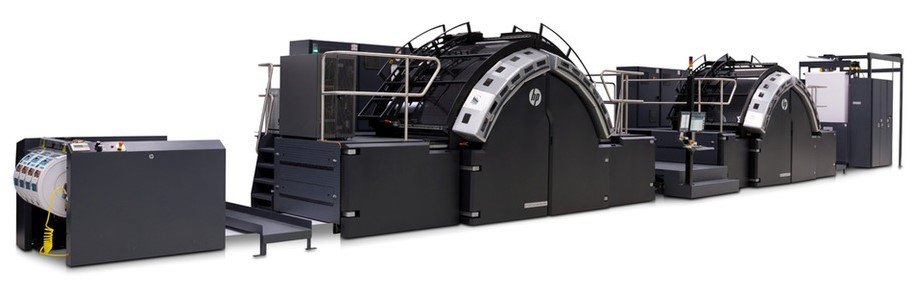
\includegraphics[width=15cm]{HP-T410}
    \caption{A HP PageWide T410 press \cite{press}}
    \label{fig:press}
\end{figure}

% Project abstract summarizing the entire document in 100-150 words.
\bigskip
\bigskip
\begin{abstract}
HP has a line of industrial printing presses that can be fairly difficult to operate, often requiring well-trained staff to choose the correct settings for large printing jobs. The ramifications of failing to set up a job properly are expensive, with a large amount of paper potentially being wasted. A proposed solution to reduce the time spent choosing settings and the amount of paper waste is to use an automation framework that utilizes machine reasoning. This framework will take a number of inputs, such as document length and paper size, to produce optimal settings for that printing job. It will provide a justification for all of the settings, and be able to take feedback from the press operator. It will be able to use the feedback in reasoning for future jobs. 
\end{abstract}

% Definition and description of the problem you are trying to solve written for a general, but educated audience
\pagebreak
\section{Problem Definition}
HP's Corvallis site produces PageWide Web Presses, multi-million-dollar printing presses larger than a shipping container that print from large rolls of paper at up to 16 feet per second. Extensive knowledge of the product is required to ensure that jobs and press settings are correctly prepared for printing. If jobs and press settings are not correctly set up, they may result in tons of wasted paper. Setting a job up correctly typically requires well-trained staff with a lot of expertise. Since such staff is expensive and difficult to train, HP is looking to remove the human element, opting instead for automation to choose the correct settings and operating procedures. This project will deal with working to implement said automation using a machine-reasoning engine.

% Proposed solution
\bigskip
\section{Proposed Solution}
In order to develop an automated system, we have to fully understand the input we are getting and the existing settings we are going to use. The system takes two different types of files, XML and PDF. We have to extract both of these files to get the characteristics we need. These characteristics will impact things like the type of paper to use, the printing speed, the heat and speed of the dryer, and so on. There isn’t a specific technology we are going to use. Basically, this project is related to maching-reasoning, so we need to have a server that we can test our system — our client should also have access to the server so they can see what we are working on. Eventually we will use a real-world press to test the results. HP will provide us the machine we will be using in their campus in Corvallis.\\

The eventual goal of this project is to produce a maching-reasoning engine — and a user interface for interacting with said engine — to analyze the input files for a print job and output a profile of settings that best fits its needs. The maching-reasoning engine will sit between the print job queue, which holds all of the jobs that HP will execute on a given day, and an existing internal tool used for creating the jobs. The engine will determine the best settings along with a justification for why each setting was chosen. If a job is deemed incomplete or not fit for printing, the engine will not place it in the queue.\\

HP will provide us several white papers written by their research team a few years ago, containing information related to best-practices and the optimal settings to use depending on the contents of the print job. So, we will have to digest it and apply the idea to a real-world product. In other words, we have to develop our system based on the knowledge we learned from those papers. After we come out with a prototype, the experts at HP will provide feedback to us based on their real-world experience on the project and production. Therefore we can prevent critical errors before real-world testing. Ideally, we should use the language similar to what HP used to develop its current system. But since it’s an experimental project, we are more focusing on usability instead of compatibility.\\

During the system designing process, we will need to ask some professors at OSU and some senior engineers at HP for help. The system will be a cloud API based maching-reasoning engine that will generate the ideal press settings or examine the setting from the client. The system will be used in two areas. First is to integrate it with the current press system. Second is a responsive web-application. The web-application will separate the printing process into three categories: upload files; choose the settings; view printing results. All of these steps can be done by different users. The application will have a simplified setting selection so it is more friendly for the general users. Due to the experimental nature of this project, it’s not guaranteed the system will work eventually but the chance of success is fairly high.

% Performance metrics: Tell how you will know when you have completed the project. Metrics help you and your client agree on what successful completion (e.g., % faster, $-amount cheaper, easier to use, "a working prototype," a complete white paper with research results) of the project looks like.
\bigskip
\section{Performance Metrics}
The success of the project will be measured in a few different ways. The overall performance of the automation will be judged by the increase in productivity, consisting of a decrease in the amount of time required to set up a printing job in addition to a reduction in the amount of waste paper. Another factor that will be looked at is the amount of money saved, not only as a result of automation (that is, having less employees on payroll), but also as a result of using less paper for the printing job.

A "successful completion" of the project means that a working prototype has been created. In reality, the project may never be truly "complete," as the prototype will have functionality added to it over many iterations, which may occur outside of the context of this project. Within the context of the project, our team is expected to deliver a working prototype that is modular, so that these additions may be made at a later time.

\bigskip
\begin{thebibliography}{1}
\bibitem{press}
“HP PageWide Industrial presses,” HP PageWide Industrial presses | HP® Official Site. [Online]. Available: https://www8.hp.com/us/en/commercial-printers/pagewide-industrial/products.html. [Accessed: 21-Oct-2019].
\end{thebibliography}

\end{document}